% ========== Template by IC\M/T Institute of Creative\Media/Technologies =============
% ==========  M. Wagner and K. Blumenstein, N. Thuer 2017         ============= 
% ==========  Based on the LaTeX Thesis Template for the University of Applied Sciences St.Pölten by P. Lechner https://github.com/hrtlacek/ThesisTemplate-FH-StP        ============= 


%Dokumentklasse without end dot ;-)
\documentclass[a4paper,11pt, numbers=noenddot]{scrreprt}
\usepackage[left= 3.5cm,right = 3cm, bottom = 3.5 cm, top = 3 cm]{geometry}
\usepackage[onehalfspacing]{setspace}

% ============= Settings for the Work =============

\def\workTitle{<Title of the Work>}
\def\subTitle{<Subtitle of the Work>}
\def\specialization{<Specialization>}
\def\studentFirstName{<FirstName>}
\def\studentLastName{<LastName>}
\def\studentId{<StudentID>}
\def\advisorPreTitle{<Pre-Title>}
\def\advisoFirstName{<FirstName>}
\def\advisorLastName{<LastName>}
\def\advisorPosTitle{<Pos-Title>}
\def\assessorPreTitle{<Pre-Title>}
\def\assessorFirstName{<FirstName>}
\def\assessorLastName{<LastName>}
\def\assessorPosTitle{<Pos-Title>}
\def\place{<Place>}
\def\dateDay{<DD>}
\def\dateMonth{<MM>}
\def\dateYear{<YYYY>}
% Switch between German and English version!!! 
\newif\ifuseGermanVersion	% <== DONT TOUCH THIS!!!
% To switch the version please use the comment "%" option :-). After a language change, jou have to rebuild the whole project (in Overleaf --> recompile from scratch) 
%\useGermanVersiontrue		% German version
\useGermanVersionfalse		% English version

% ============= Packages =============

% Dokumentinformationen
\usepackage[
	pdftitle={\workTitle},
	pdfsubject={},
	pdfauthor={\studentFirstName \studentLastName},
	pdfkeywords={}
	pdftex=true, 
	colorlinks=true,
 	breaklinks=true,
	citecolor=black,
	linkcolor=black,	
	menucolor=black,	
	urlcolor=black
]{hyperref}

\hypersetup{
    bookmarks=true,         % show bookmarks bar?
    unicode=false,          % non-Latin characters in Acrobat’s bookmarks
    pdftoolbar=true,        % show Acrobat’s toolbar?
    pdfmenubar=true,        % show Acrobat’s menu?
    pdffitwindow=false,     % window fit to page when opened
    pdfstartview={FitH},    % fits the width of the page to the window
    pdftitle={My title},    % title
    pdfauthor={Author},     % author
    pdfsubject={Subject},   % subject of the document
    pdfcreator={Creator},   % creator of the document
    pdfproducer={Producer}, % producer of the document
    pdfkeywords={keyword1} {key2} {key3}, % list of keywords
    pdfnewwindow=true,      % links in new window
    colorlinks=false,       % false: boxed links; true: colored links
    linkcolor=black,          % color of internal links (change box color with linkbordercolor)
    citecolor=black,        % color of links to bibliography
    filecolor=black,      % color of file links
    urlcolor=black           % color of external links
}

% Standard Packages
\usepackage[utf8]{inputenc}

% Switch the Language
\ifuseGermanVersion
	\usepackage[ngerman]{babel}	% German
\else
	\usepackage[english]{babel} % English
\fi

\usepackage[T1]{fontenc}
\usepackage{graphicx}
\usepackage{graphicx, subfigure}
%setze pfad fuer Bilder
\graphicspath{{img/}}
\usepackage{fancyhdr}
\usepackage{lmodern}
\usepackage{color}
\usepackage{transparent}

% Citation style
\usepackage[comma,authoryear]{natbib}
%\usepackage{natbib}

% zusätzliche Schriftzeichen der American Mathematical Society
\usepackage{amsfonts}
\usepackage{mathtools}

\usepackage[export]{adjustbox}

% BlockDiagram Drawing Package
% ---tikz
\usepackage{tikz}
\usetikzlibrary{positioning}
\usepackage{pgfplots}
\pgfplotsset{compat=1.10}
\usepackage{textcomp}

%Package for using the [H] option on graphics to force them into place
\usepackage{float}

%iPython packages:
\usepackage{graphicx} % Used to insert images
\usepackage{adjustbox} % Used to constrain images to a maximum size 
\usepackage{color} % Allow colors to be defined
\usepackage{enumerate} % Needed for markdown enumerations to work
\usepackage{geometry} % Used to adjust the document margins
\usepackage{amsmath} % Equations
\usepackage{amssymb} % Equations
\usepackage[mathletters]{ucs} % Extended unicode (utf-8) support
% \usepackage[utf8x]{inputenc} % Allow utf-8 characters in the tex document
\usepackage{fancyvrb} % verbatim replacement that allows latex
\usepackage{grffile} % extends the file name processing of package graphics 
                         % to support a larger range 
    % The hyperref package gives us a pdf with properly built
    % internal navigation ('pdf bookmarks' for the table of contents,
    % internal cross-reference links, web links for URLs, etc.)
\usepackage{hyperref}
\usepackage{longtable} % longtable support required by pandoc >1.10

% embedding of audio/video files etc.
% \usepackage{attachfile}
% \usepackage{movie15}
% \usepackage{media9}
% \usepackage{menukeys}

\usepackage[labelfont=it, labelsep=period, format=plain,justification=raggedright, singlelinecheck=false]{caption}
\captionsetup[figure]{justification=centering}
\definecolor{light-gray}{gray}{0.85}

% Switch between German and English based on the Settingx.tex. file
\usepackage{ifthen}

%\captionsetup[listing]{
%  labelsep = newline,
%  textfont = sc, 
%  name = LISTING, 
%  justification=justified,
%  singlelinecheck=false,%%%%%%% a single line is centered by default
%  labelsep=colon,%%%%%%
%  skip = \medskipamount}

% =============== BlockDiagram Drawing Config
\usetikzlibrary{shapes,arrows}

% Definition of blocks:
\tikzset{%
  block/.style    = {draw, thick, rectangle, minimum height = 3em,
    minimum width = 3em},
  sum/.style      = {draw, circle, node distance = 2cm}, % Adder
  input/.style    = {coordinate}, % Input
  output/.style   = {coordinate}, % Output
  mult/.style	  = {draw, isosceles triangle, minimum height=1cm, minimum width =1cm}
}
%mult/.style	  = {isosceles triangle, sharp corners, anchor=center, xshift=-4mm, minimum height=1.5cm, minimum width =0.05cm}
%isosceles triangle, fill=gray!25, minimum width=1.5cm

% Defining string as labels of certain blocks.
\newcommand{\suma}{\Large$+$}
\newcommand{\inte}{$\displaystyle \int$}
\newcommand{\derv}{\huge$\frac{d}{dt}$}
\newcommand{\conv}{\huge$\ast$}

% ============================================

% -- Settings für Code abbildungen
\usepackage{listings,lstautogobble}
\lstset{backgroundcolor=\color{light-gray},frame=single, framerule=0pt, showspaces=false, showtabs=false, numbers=left, numbersep=5pt, breaklines=false, autogobble=true, language=C++}

% Setze arial font
\usepackage[scaled]{uarial}
\renewcommand*{\familydefault}{\sfdefault}

% FH-grünBlau
\definecolor{FH}{rgb}{0.10, 0.57, 0.68}
% FH-grünBlau 2
\definecolor{FH2}{rgb}{0.0392, 0.666, 0.549}


% nicht einrücken nach Absatz
\setlength{\parindent}{0pt}

% Paragraph-Abstand
\setlength{\parskip}{0.5em}

% ============= Kopf- und Fußzeile =============

%\renewcommand{\headrulewidth}{0.4pt}
%\renewcommand{\footrulewidth}{0pt}

\renewcommand{\chaptermark}[1]{\markboth{\thechapter~ #1}{}}

\fancypagestyle{icmt-fancy}{%
  \fancyhf{}% Clear header and footer
  \fancyhead[L]{\leftmark}
  \fancyfoot[R]{\thepage}% Custom footer
  \renewcommand{\headrulewidth}{0.4pt}% Line at the header visible
  \renewcommand{\footrulewidth}{0.0pt}% Line at the footer visible
}

% Redefine the plain page style
\fancypagestyle{plain}{%
  \fancyhf{}%
  \fancyfoot[R]{\thepage}%
  \renewcommand{\headrulewidth}{0pt}% Line at the header invisible
  \renewcommand{\footrulewidth}{0.0pt}% Line at the footer visible
}

% ============= Package Einstellungen & Sonstiges ============= 

%Besondere Trennungen
\hyphenation{De-zi-mal-tren-nung St-rei-fen-licht-scan-nern}

%römische Aufzählungen mit \RM{Zahl}
\newcommand{\RM}[1]{\MakeUppercase{\romannumeral #1}}

% ============= Dokumentbeginn =============

\begin{document}

% Select the right main page ;-)
\ifuseGermanVersion
	
% setup page dimensions for titlepage
\newgeometry{left=2.4cm,right=2.4cm,bottom=2.5cm,top=2cm}

% force baselineskip and parindent
%\newlength{\tmpbaselineskip}
%\setlength{\tmpbaselineskip}{\baselineskip}
%\setlength{\baselineskip}{13.6pt}
%\newlength{\tmpparindent}
%\setlength{\tmpparindent}{\parindent}
%\setlength{\parindent}{17pt}

% first titlepage
\pagestyle{empty}

\begin{figure}[H]
\vspace*{-2.5cm}
\hspace*{2.5cm}

\includegraphics[keepaspectratio, width=1.4\textwidth, right]{TemplateElements/fhLogo3.png}
\end{figure}



\begin{center}

\vspace{1cm}

\begin{minipage}[t][5cm][s]{\textwidth}%
\centering
\Huge{{\color{FH2}{\fontsize{24}{30} \selectfont \workTitle\\}}}
\vspace{0.5cm}
\LARGE{{\color{FH2}{\fontsize{16}{24} \selectfont \subTitle\\}}}
\end{minipage}

\vspace{1cm}


\LARGE{Diplomarbeit}


\vspace{1.5cm}

\fontsize{11pt}{15pt}\selectfont Ausgef\"uhrt zum Zweck der Erlangung des akademischen Grades\\
\textbf{Dipl.-ing.f\"ur technisch-wissenschaftliche Berufe}

\vspace{6mm}

am Masterstudiengang Digitale Medientechnologien an der\\ 
Fachhochschule St. P\"olten, \textbf{Vertiefungsrichtung \specialization} 

\vspace{1.5cm}

Ausgef\"uhrt von:\\ 
\fontsize{15pt}{15pt}\selectfont
\textbf{\studentFirstName\ \studentLastName} \\
\fontsize{11pt}{15pt}\selectfont
\studentId

\vspace{2cm}

\begin{tabular}{lll}
Betreuer and Erstbegutachter: & \advisorPreTitle\ \advisoFirstName\ \advisorLastName, \advisorPosTitle\\
Zweitbegutachter: & \assessorPreTitle\ \assessorFirstName\ \assessorLastName, \assessorPosTitle\\
\end{tabular}

\vspace{2cm}


\large{\place, \dateDay.\dateMonth.\dateYear}


\end{center}

\restoregeometry
\else
	
% setup page dimensions for titlepage
\newgeometry{left=2.4cm,right=2.4cm,bottom=2.5cm,top=2cm}

% force baselineskip and parindent
%\newlength{\tmpbaselineskip}
%\setlength{\tmpbaselineskip}{\baselineskip}
%\setlength{\baselineskip}{13.6pt}
%\newlength{\tmpparindent}
%\setlength{\tmpparindent}{\parindent}
%\setlength{\parindent}{17pt}

% first titlepage
\pagestyle{empty}

\begin{figure}[H]
\vspace*{-2.5cm}
\hspace*{2.5cm}

\includegraphics[keepaspectratio, width=1.4\textwidth, right]{TemplateElements/fhLogo3.png}
\end{figure}



\begin{center}

\vspace{1cm}

\begin{minipage}[t][5cm][s]{\textwidth}%
\centering
\Huge{{\color{FH2}{\fontsize{24}{30} \selectfont \workTitle\\}}}
\vspace{0.5cm}
\LARGE{{\color{FH2}{\fontsize{16}{24} \selectfont \subTitle\\}}}
\end{minipage}

\vspace{1cm}

\ifuseBachelorMediaTechnologiesOne
	\LARGE{Research Paper}
\else
	\ifuseBachelorMediaTechnologiesTwo
		\LARGE{Bachelor Thesis}
\else
	\ifuseMasterDigitalMediaTechnologies
		\LARGE{Diploma Thesis}
\else
	\ifuseMasterDigitalHealthCare
		\LARGE{Master Thesis}
    \else
        \LARGE{YOU HAVE TO CHOOSE THE PROGRAM TYPE IN THE SETTINGS!!!}
  	\fi
\fi
\fi
\fi
  
\vspace{1.3cm}
\ifuseBachelorMediaTechnologiesOne
	\fontsize{11pt}{15pt}\selectfont Bachelor Course on Media Technology\\
at St. Pölten University of Applied Sciences\\  
\else
	\ifuseBachelorMediaTechnologiesTwo
		\fontsize{11pt}{15pt}\selectfont Bachelor Course on Media Technology\\
at St. Pölten University of Applied Sciences\\  
\else
	\ifuseMasterDigitalMediaTechnologies
		\fontsize{11pt}{15pt}\selectfont For attainment of the academic degree of\\
		\textbf{Dipl.-ing.für technisch-wissenschaftliche Berufe}
\else
	\ifuseMasterDigitalHealthCare
    	\fontsize{11pt}{15pt}\selectfont For attainment of the academic degree of\\
		\textbf{Master of Science in Engineering (MSc)}
    \else
        \LARGE{YOU HAVE TO CHOOSE THE PROGRAM TYPE IN THE SETTINGS!!!}
  	\fi
\fi
\fi
\fi

\vspace{4mm}
 
\ifuseMasterDigitalMediaTechnologies
	in the Masters Course Digital Media Technologies at St. Pölten\\ 
University of Applied Sciences, \textbf{specialized area \specialization}
\else
	\ifuseMasterDigitalHealthCare
		in the Masters Course Digital Healthcare\\ 
at St. Pölten University of Applied Sciences
    \else
  	\fi
\fi





\vspace{1.3cm}

Submitted by:\\ 
\fontsize{15pt}{15pt}\selectfont
\textbf{\studentFirstName\ \studentLastName} \\
\fontsize{11pt}{15pt}\selectfont
\studentId

\vspace{1.8cm}
\ifuseBachelorMediaTechnologiesOne
	\begin{tabular}{lll}
    Advisor: & & \advisorPreTitle\ \advisoFirstName\ 		\advisorLastName, \advisorPosTitle\\
    %Zweitbegutachter/in: & & [Titel Vorname Zuname]
    \end{tabular}
\else
	\ifuseBachelorMediaTechnologiesTwo
		\begin{tabular}{lll}
        Advisor: & & \advisorPreTitle\ \advisoFirstName\ \advisorLastName, \advisorPosTitle\\
        %Zweitbegutachter/in: & & [Titel Vorname Zuname]
		\end{tabular}
\else
  \begin{tabular}{lll}
  Advisor and First Assessor: & \advisorPreTitle\ \advisoFirstName\ \advisorLastName, \advisorPosTitle\\
  Second Assessor: & \assessorPreTitle\ \assessorFirstName\ \assessorLastName, \assessorPosTitle\\
  \end{tabular}

\fi
\fi

\vspace{1.8cm}


\large{\place, \dateDay.\dateMonth.\dateYear}


\end{center}

\restoregeometry
\fi

% \part im Inhaltsverzeichnis nicht nummerieren
\makeatletter
\let\partbackup\l@part
\renewcommand*\l@part[2]{\partbackup{#1}{}}

%Seitennummerierung neu beginnen, Zahlen [arabic], röm.Zahlen [roman,Roman], Buchstaben [alph,Alph]
\pagenumbering{Roman}

\newpage
\ifuseGermanVersion
	\chapter*{Ehrenwörtliche Erklärung}
\label{ch:erklaerung}
% \begin{flushleft}
% 	test
% \end{flushleft}

\begin{flushleft}
Ich versichere, dass 
\end{flushleft}

\begin{flushleft}
- ich diese Bachelorarbeit selbständig verfasst, andere als die angegebenen Quellen und Hilfsmittel nicht benutzt und mich sonst keiner unerlaubten Hilfe bedient habe.
\end{flushleft}

\begin{flushleft}
- ich dieses Bachelorarbeitsthema bisher weder im Inland noch im Ausland einem Begutachter/ einer Begutachterin zur Beurteilung oder in irgendeiner Form als Prüfungsarbeit vorgelegt habe.	
\end{flushleft}

\begin{flushleft}
- diese Arbeit mit der vom Begutachter/von der Begutachterin beurteilten Arbeit übereinstimmt. \\[1.5cm]	
\end{flushleft}
% - diese Arbeit mit der vom Begutachter/von der Begutachterin beurteilten Arbeit übereinstimmt. \\
% \\[1.5cm]
Datum:	\hrulefill\enspace Unterschrift: \hrulefill
\\[3.5cm]
\else
	\chapter*{Declaration}
\label{ch:declaration}

\begin{flushleft}
- The attached research paper is my own, original work undertaken in partial fulfillment of my degree.
\end{flushleft}

\begin{flushleft}
- I have made no use of sources, materials or assistance other than those which habe been openly and fully acknowledged in the text. If any part of another person’s work has been quoted, this either appears in inverted commas or (if beyond a few lines) is indented.
\end{flushleft}

\begin{flushleft}
- Any direct quotation or source of ideas has been identified in the text by author, date, and page number(s) immediately after such an item, and full details are provided in a reference list at the end of the text.
\end{flushleft}

\begin{flushleft}
- I understand that any breach of the fair practice regulations may result in a mark of zero for this research paper and that it could also involve other repercussions.
\end{flushleft}

\vspace{1.5cm}

Date:	\hrulefill\enspace Signature: \hrulefill
\\[3.5cm]
\fi

\newpage
%\chapter*{Kurzfassung}
%\label{ch:kurzfassung}
%Dies ist die Kurzfassung der Arbeit. Lorem ipsum dolor sit amet, consectetur adipisicing elit, sed do eiusmod
%tempor incididunt ut labore et dolore magna aliqua. Ut enim ad minim veniam,
%quis nostrud exercitation ullamco laboris nisi ut aliquip ex ea commodo
%consequat. Duis aute irure dolor in reprehenderit in voluptate velit esse
%cillum dolore eu fugiat nulla pariatur. Excepteur sint occaecat cupidatat non
%proident, sunt in culpa qui officia deserunt mollit anim id est laborum.


%\newpage

\chapter*{Abstract}
\label{ch:abstract}

Introduction: Warum behandeln wir das Thema

Purpose: Welches Problem soll gelöst werden

Method: Wie wurde die Problemlösung gemacht

Product: Was war das Ergebnis

Conclusion: Was sind die Folgerungen / Schlussfolgerungen aus den gewonnen Erkenntnissen

keine Referenzen und Zitate


\chapter*{Kurzfassung}
\label{ch:kurzfassung}

Das Abstract auf deutsch.

\newpage

%Inhaltsverzeichnis
\tableofcontents

\newpage
%Seitennummerierung neu beginnen, Zahlen [arabic], röm.Zahlen [roman,Roman], Buchstaben [alph,Alph]
\pagenumbering{arabic}

% pagestyle für gesamtes Dokument aktivieren
\pagestyle{icmt-fancy}
\newpage

% /*================================
% =            EXAMPLE            =
% ================================*/

% Delete this include at the end
\chapter{Example}
\label{ch:example}

!!! Please delete this chapter after finishing your work !!!

\section{Settings}

To add your name and the title of your work, please use the ``Settings.tex'' file!
Additionally, switch there between German and English version.

\section{How to Make Sections and Subsections}

Use section and subsection commands to organize your document. \LaTeX{} handles all the formatting and numbering automatically. Use ref and label commands for cross-references.

\subsection{How to Make Lists}

You can make lists with automatic numbering \dots

\begin{enumerate}
\item Like this,
\item and like this.
\end{enumerate}
\dots or bullet points \dots
\begin{itemize}
\item Like this,
\item and like this.
\end{itemize}
\dots or with words and descriptions \dots
\begin{description}
\item[Word] Definition
\item[Concept] Explanation
\item[Idea] Text
\end{description}\section{Section}

You have to write text between each headline.

\section{Citation}

This part describes the 3 types of citations which are possible:

\section{Direct Citation}

The maximum for a direct citation is a ${1/2}$ page.

\begin{quotation}
	Overview first, zoom and filter, then details-on-demand~\citep{shneiderman_eyes_1996}
\end{quotation}

\section{Floating Text Citation}

\citet{shneiderman_eyes_1996} defined the Visual Information Seeking Mantra as ``Overview first, zoom and filter, then details-on-demand''. 
\citep{kahneman_thinking_2012}

\section{Indirect Citation}

Some text which summarizes a paper or a book chapter. This could take several lines~\citep{shneiderman_eyes_1996}. 

\newpage
\section{Figures}

To place a figure use the following code example

\begin{figure}[ht!]
  \centering
  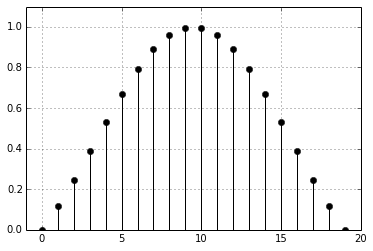
\includegraphics[width=1\columnwidth]{Figures/Example}
  \caption{Interactive data exploration with multiple devices.}
  \label{fig:example}
\end{figure}

Refer to a figure in the following forms:\\
If you take a look at Figure~\ref{fig:example} ...\\
... text text (see Figure~\ref{fig:example}) ...

\section{Listings}
\begin{lstlisting}[caption=A bit of source code., label=lst:test]
if( true == questions )
{
    std::cout << "Let me google it for you";
}
else
{
    std::cout << "Great";
}
\end{lstlisting}

Now lets take a look at Listing~\ref{lst:test}.

\newpage
\section{Table}

\begin{table}[ht!]
  \caption{My caption with a very useful description. die kann auch etwas länger sein und über mehrere Zeilen gehen und so weiter.}
  \label{my-label}
  \begin{tabular}{llr}
    \hline
    \multicolumn{2}{c}{Item} &            \\ \cline{1-2}
    Animal     & Description & Price (\$) \\ \hline
    Gnat       & per gram    & 13.65      \\
               & each        & 0.01       \\
    Gnu        & stuffed     & 92.50      \\
    Emu        & stuffed     & 33.33      \\
    Armadillo  & frozen      & 8.99       \\ \hline
  \end{tabular}
\end{table}

For the fast generation of tables from Excel use \url{http://www.heise.de/download/excel2latex.html}

\section{Equations}

\LaTeX{} is great at typesetting equations. Let $X_1, X_2, \ldots, X_n$ be a sequence of independent and identically distributed random variables with $\text{E}[X_i] = \mu$ and $\text{Var}[X_i] = \sigma^2 < \infty$, and let

$$S_n = \frac{X_1 + X_2 + \cdots + X_n}{n}$$

This was a equation without a label.
      
\begin{equation}
S_n = \frac{1}{n}\sum_{i}^{n} X_i
\label{eq:test}
\end{equation}


This is the reference to equation~\ref{eq:test}.      


denote their mean. Then as $n$ approaches infinity, the random variables $\sqrt{n}(S_n - \mu)$ converge in distribution to a normal $\mathcal{N}(0, \sigma^2)$.




% /*================================
% =            CONTENTS            =
% ================================*/

\chapter{Introduction / Einleitung}
\label{ch:introduction}

Führt in die Thematik, Problem- und Aufgabenstellung ein

Vorstellung der Forschungsfrage

Enthält Grundlagenwissen

Gibt Überblick über die Arbeit

Darstellung der Related Work - sofern bereits ähnliche Arbeiten zu diesem Themengebiet existieren; In aller Kürze: Was gibt es? Was sind die Ergebnisse? Ist etwas offen geblieben? Fehlt etwas?

\chapter{Method / Methode}
\label{ch:method}

Wie wurde Literatur gefunden?

Welche Journals, Conferences, Libraries, Search engines… wurden genutzt?

Nach welchen Keywords wurde gesucht, wie viele Treffer gab es?

Nach welchen Kriterien wurde selektiert und warum?

\chapter{Results}
\label{ch:results}

Presenting found literature in a useful way

\section{First Section}
Ich bin Text, Text, Text\footnote{\url{http://mfg.fhstp.ac.at}}


\subsection{First Subsection}
\chapter{Discussion}
\label{ch:discussion}

Comparison of presented technologies/methods/projects

Kritische Diskussion / Vergleich der Ansätze

Welche Methoden werden zumeist genutzt, warum?

Überblick / Zusammenfassung der gefundenen Literatur in einer sinnvollen Kategorisierung / Charakterisierung

\chapter{Conclusion}
\label{ch:conclusion}

Was kann man daraus lernen?

Was fehlt?

Ideen für zukünftige Forschung

\pagestyle{plain} 

%Literaturverzeichnis
\bibliographystyle{apalike}
\bibliography{Bibliography.bib}

% Bilderverzeichnis
\newpage
\listoffigures
% Tableverzeichnis
\newpage
\listoftables
%Codelistingsverzeichnis
\newpage
\lstlistoflistings
\newpage

% ============================================


\chapter*{Appendices}

\addcontentsline{toc}{chapter}{Appendices}
\renewcommand{\thesection}{\Alph{section}}

\section{Appendix}
\label{appendix_a}

LoHrem ipsum dolor sit amet, consectetur adipisicing elit, sed do eiusmod
tempor incididunt ut labore et dolore magna aliqua. Ut enim ad minim veniam,
quis nostrud exercitation ullamco laboris nisi ut aliquip ex ea commodo
consequat. Duis aute irure dolor in reprehenderit in voluptate velit esse
cillum dolore eu fugiat nulla pariatur. Excepteur sint occaecat cupidatat non
proident, sunt in culpa qui officia deserunt mollit anim id est laborum.LoHrem ipsum dolor sit amet, consectetur adipisicing elit, sed do eiusmod
tempor incididunt ut labore et dolore magna aliqua. Ut enim ad minim veniam,
quis nostrud exercitation ullamco laboris nisi ut aliquip ex ea commodo
consequat. Duis aute irure dolor in reprehenderit in voluptate velit esse
cillum dolore eu fugiat nulla pariatur. Excepteur sint occaecat cupidatat non
proident, sunt in culpa qui officia deserunt mollit anim id est laborum.
LoHrem

\newpage

\section{Appendix}
\label{appendix_b}

LoHrem ipsum dolor sit amet, consectetur adipisicing elit, sed do eiusmod
tempor incididunt ut labore et dolore magna aliqua. Ut enim ad minim veniam,
quis nostrud exercitation ullamco laboris nisi ut aliquip ex ea commodo
consequat. Duis aute irure dolor in reprehenderit in voluptate velit esse
cillum dolore eu fugiat nulla pariatur. Excepteur sint occaecat cupidatat non
proident, sunt in culpa qui officia deserunt mollit anim id est laborum.LoHrem ipsum dolor sit amet, consectetur adipisicing elit, sed do eiusmod
tempor incididunt ut labore et dolore magna aliqua. Ut enim ad minim veniam,
quis nostrud exercitation ullamco laboris nisi ut aliquip ex ea commodo
consequat. Duis aute irure dolor in reprehenderit in voluptate velit esse
cillum dolore eu fugiat nulla pariatur. Excepteur sint occaecat cupidatat non
proident, sunt in culpa qui officia deserunt mollit anim id est laborum.
LoHrem


% ============================================

\end{document}























